\documentclass[12pt]{article}
\usepackage[utf8]{inputenc}
\usepackage[english]{babel}
\usepackage{float}
\usepackage{multicol}
\usepackage{caption}
\usepackage{subcaption}
\usepackage{graphicx}
\usepackage[margin=0.75in]{geometry}

\title{EE236: Experiment 4 -
Heart Rate Monitor}

\author{Aaron John Sabu, 170070050}

\begin{document}
\maketitle
\begin{multicols}{2}

\section{Aim of the experiment}

The experiment introduces the student to the scope of using an IR LED-phototransistor sensor (and in general sensors) and in adding circuit blocks to make the output meaningful.

\section{Methods}

The experiment was performed using a TCRT5000 IR LED-phototransistor sensor whose output was filtered initially by a high-pass filter and then a low-pass filter. Finally the final output was obtained by amplifying the output from the low-pass filter via an inverting amplifier.\\
All three op-amps required (two for the filters and one for the amplifier) were provided by one IC - LM324, a quad operational amplifier. The output was displayed on a Digital Storage Oscilloscope (DSO).\\

\begin{figure}[H]
    \centering
    \begin{subfigure}{\textwidth}
        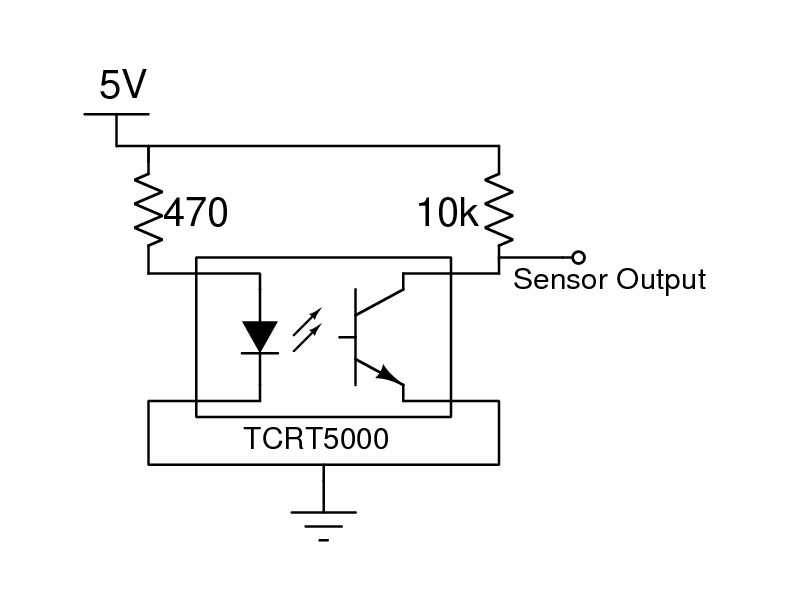
\includegraphics[width=0.5\linewidth, height=5cm]{Sensor_Circuit.png} 
        \caption{Sensor Circuit}
    \end{subfigure}\\
    \begin{subfigure}{\textwidth}
        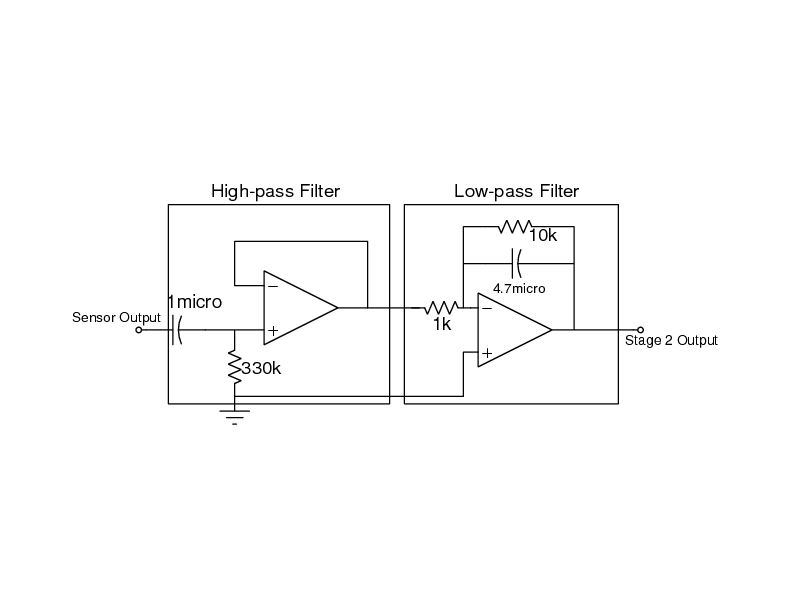
\includegraphics[width=0.5\linewidth, height=5cm]{Filters.png}
        \caption{Filters}
    \end{subfigure}\\
    \begin{subfigure}{\textwidth}
        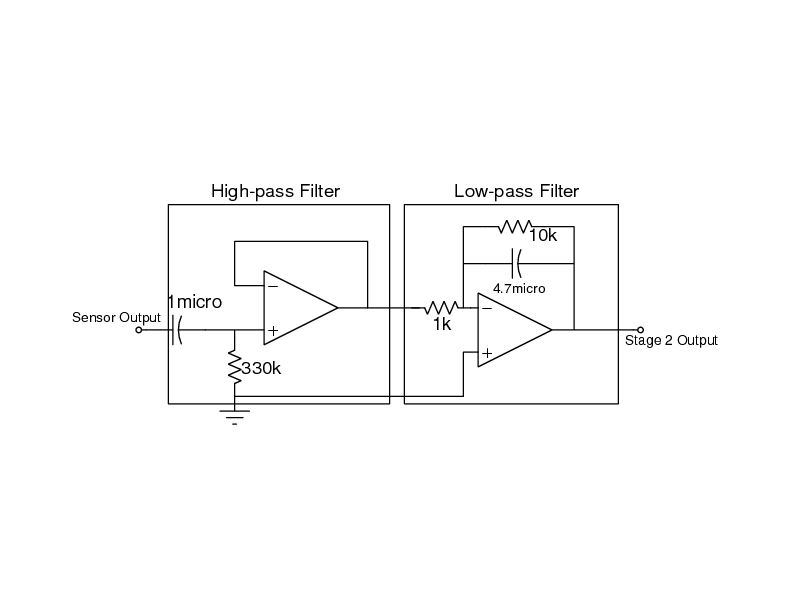
\includegraphics[width=0.5\linewidth, height=5cm]{Filters.png}
        \caption{Amplifier}
    \end{subfigure}
    \caption{Circuit Diagram}
\end{figure}

\section{Results}

\subsection{Observations}

The experiment was conducted in room temperature at approximately sea level atmospheric pressure, and the user of the apparatus was not facing any strained situations such as exercise or heavy work. Due to these factors, the heart rate is expected to be normal. 

\begin{figure}[H]
    \centering
    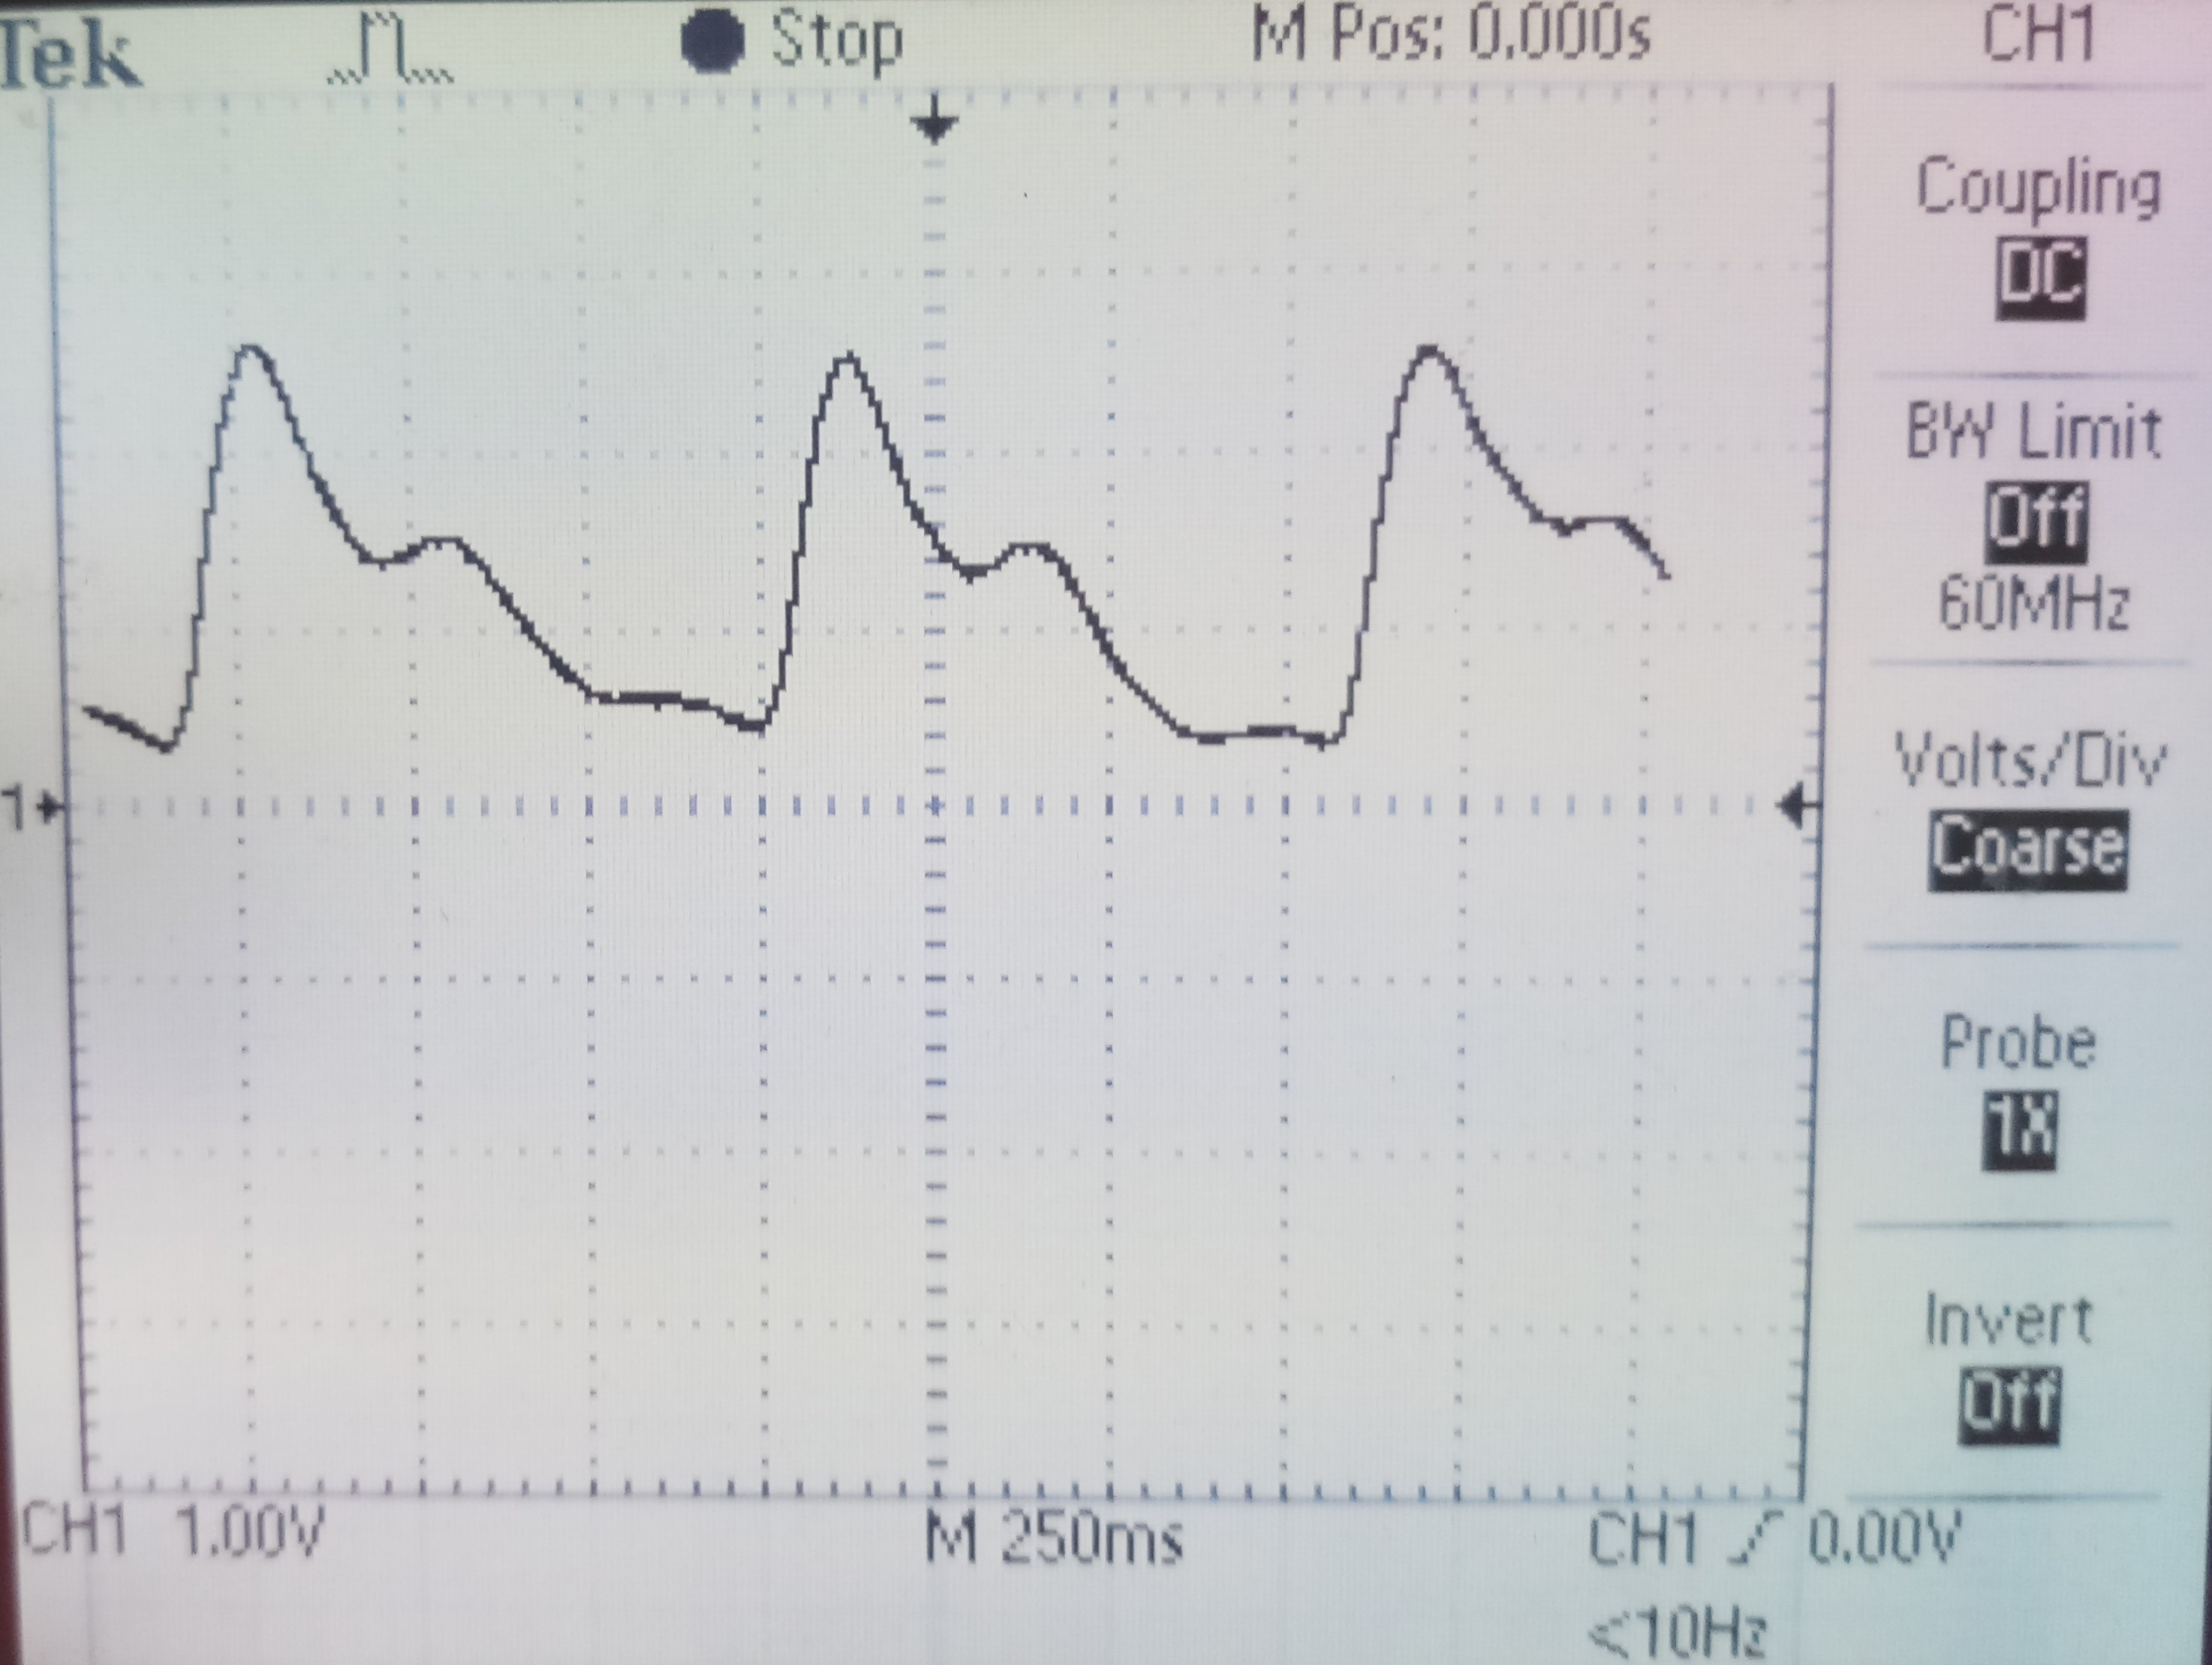
\includegraphics[width = 0.9\linewidth]{DSO_Output.jpg}
    \caption{Output from the DSO}
\end{figure}

According to the output from the DSO, the heart rate is:
\[Heart\ rate\ =\ \frac{60}{\left(250\times10^{-3}\right)\times3.4}\ =\ 70.59\ bpm\]

\subsection{Inference}

My pulse was 72 bpm when measured via a stopwatch which somewhat matches the output received on the DSO.\\
Another conclusion that can be drawn from the experiment is that the heart rate signal measured on the DSO represents the systolic peak, the dichrotic notch and finally the diastolic peak before going back to the normal state.

\section{Learning objectives}

The learning objectives were to know how to measure output from a sensor, how to remove noise from the sensor output, and how to amplify the output from the filters, hence providing an observable final output.\\
Yes, these objectives were satisfied in the case of our team. Hence we were able to observe the required output and measure the required, which was the heart rate.

\section{Quick feedback}

\subsection{What about this experiment did you find helpful?}
The fact that we used a single IC for achieving three different circuit indeed baffles me. The integration of these three circuits among each other and with the sensor circuit was indeed very helpful in the sense that I learned how we may have a very large circuit on a PCB or so and yet the circuit can be understood by dividing it into several sub-circuits.

\subsection{What about this experiment is still unclear?}
I still cannot understand the flow of light from the IR LED to the phototransistor via the finger which was placed. To my understanding, the light reflects from the blood vessel in the finger, but I do not understand how that helps in measuring the rate in which blood flows.\\
Disclaimer: My cause of non-clarity is in no way related to the course directly.

\end{multicols}
\end{document}
